% Standalone source for figures/lf_by_cell.pdf.
% Rebuild: tectonic lf_by_cell.tex   (run from report/figures/)
% Values are the LF column of Table 1 and Appendix C (results/parsing_results.md).
% A dot plot rather than bars: the axis does not start at zero, and a bar's
% length would then misrepresent the ratio between cells.
\documentclass[tikz,border=2pt]{standalone}
\usepackage{times}
\usepackage[T1]{fontenc}
\usepackage{pgfplots}
\pgfplotsset{compat=1.18}
\definecolor{cellblue}{HTML}{3D6DB3}
\definecolor{ink}{HTML}{222222}
\definecolor{inkmuted}{HTML}{6B6B6B}
\definecolor{grid}{HTML}{E2E2E2}
\begin{document}
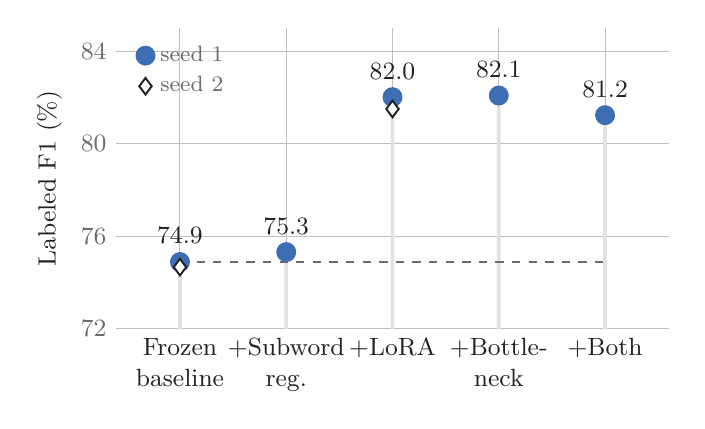
\begin{tikzpicture}
\begin{axis}[
  width=8.6cm, height=5.4cm,
  ymin=72, ymax=85,
  ytick={72,76,80,84},
  ylabel={Labeled F1 (\%)},
  ylabel style={font=\small, color=ink},
  symbolic x coords={Baseline, Subword, LoRA, Bottleneck, Both},
  xtick={Baseline, Subword, LoRA, Bottleneck, Both},
  xticklabel style={font=\small, color=ink},
  x tick label style={text width=1.6cm, align=center},
  xticklabels={Frozen\\baseline, +Subword\\reg., +LoRA, +Bottle-\\neck, +Both},
  yticklabel style={font=\small, color=inkmuted},
  ymajorgrids, grid style={grid},
  axis line style={draw=none},
  tick style={draw=none},
  enlarge x limits=0.15,
  clip=false,
  legend style={font=\footnotesize, draw=none, fill=none, at={(0.02,0.98)}, anchor=north west, text=inkmuted},
  legend cell align=left,
]
% stems from the baseline level, to make the deltas readable
\addplot[ybar, bar width=1.4pt, fill=grid, draw=none, forget plot, ybar legend]
  coordinates { (Baseline,74.89) (Subword,75.32) (LoRA,82.02) (Bottleneck,82.09) (Both,81.24) };
\addplot[only marks, mark=*, mark size=3.4pt, color=cellblue,
  nodes near coords, point meta=explicit symbolic,
  every node near coord/.append style={font=\small, color=ink, yshift=3pt}]
  coordinates {
    (Baseline,74.89)   [74.9]
    (Subword,75.32)    [75.3]
    (LoRA,82.02)       [82.0]
    (Bottleneck,82.09) [82.1]
    (Both,81.24)       [81.2]
  };
\addlegendentry{seed 1}
\addplot[only marks, mark=diamond*, mark size=3pt, color=ink, fill=white, line width=0.7pt]
  coordinates { (Baseline,74.67) (LoRA,81.51) };
\addlegendentry{seed 2}
% dashed baseline level
\draw[dashed, color=inkmuted, line width=0.5pt]
  (axis cs:Baseline,74.89) -- (axis cs:Both,74.89);
\end{axis}
\end{tikzpicture}
\end{document}
